\section{Related Works}

\noindent\textbf{Vision-Language-Action Models}
Vision-language models (VLMs) \citep{liu2023visual,wang2024cogvlm} have demonstrated strong performance in image-related and cross-modal tasks. Leveraging these capabilities, vision-language-action (VLA) models further finetune VLMs on large-scale robotic datasets \citep{vuong2023open,liu2023libero}, which usually consist of extensive human demonstrations. At each timestep, VLAs \citep{black2024pi0visionlanguageactionflowmodel,intelligence2025pi05visionlanguageactionmodelopenworld,kim2024openvla,li2024cogact,qu2025spatialvla} usually take the current environment observation (image) and a language instruction as inputs, and are trained to output actions of the next step. Although they have demonstrated high performance on certain benchmarks, due to the large parameters, they are 1) inefficient in rollout and 2) unable to incorporate historical frames in the context. In contrast, our model, by disentangling the static and dynamic components, is efficient in inference by leveraging the KV-cache of static components, and is able to incorporate a long history for temporally dependent tasks. 
\begin{figure}[t]
    \centering
    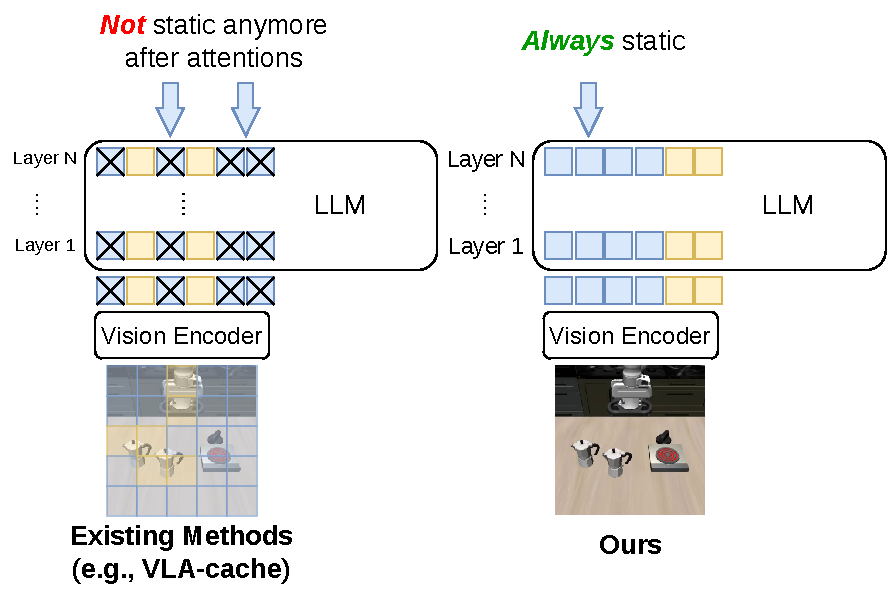
\includegraphics[width=0.8\linewidth]{figs/related_work1.pdf}
    \caption{Some of the existing methods \citep{xu2025vla,liu2025ttf} that exploit to reuse information in previous frames ignore the problem that the static patches will be affected by attentions even if they are identical in the original pixel space.}
    \label{fig:related_work1}
    % \vspace{-1em}
\end{figure}

\noindent\textbf{VLA Acceleration}
Methods to improve VLA's efficiency usually focus on general quantization or pruning methods. For example, \citet{kim2024openvla,reddy2019sqilimitationlearningreinforcement,park2024quantizationawareimitationlearningresourceefficientrobotic} explores quantization techniques applied to VLAs. \citet{shukor2025smolvlavisionlanguageactionmodelaffordable,yang2025efficientvla,zhang2025mole,yue2024deer} explored pruning unimportant tokens and layers according to some heuristics. Although reducing the computational complexity of VLAs, these methods just migrate acceleration methods from existing general machine learning models, thus totally ignoring the unique characteristics of VLAs. Different from these methods, recent works \citep{xu2025vla,liu2025ttf,tan2025think} explore temporal redundancy in decision making: consecutive frames share temporal correlation, enabling avoiding recomputation of some components by, for example, leveraging the KV-cache of previous steps. However, these methods rely on non-learnable heuristics to recache or simply reuse the previous action, which may suffer from suboptimal performance. Notably, some of these methods \citep{xu2025vla,liu2025ttf} implicitly assume that visual similarity in pixel space implies invariance in the latent representations produced by the vision encoder and LLM—an assumption that does not generally hold in transformer-based architectures, as illustrated in Figure~\ref{fig:related_work1}.

\noindent\textbf{Multi-Frame VLAs}
Existing approaches to incorporating historical frames in VLAs typically provide the model with only indirect or compressed access to temporal information. For example, \citet{jang2025contextvla} uses a non-learnable pooling operation to condense historical frames into a fixed number of tokens. \citet{liu2025ttf,torne2026mem} incorporate historical frames into the current input via patch-wise mixing. TraceVLA \citep{zheng2024tracevla} overlays visual traces of keypoints onto the current observation to indicate object trajectories. In addition, MemoryVLA \citep{shi2025memoryvlaperceptualcognitivememoryvisionlanguageaction} exposes the LLM backbone to only a single frame at each timestep and delegates multi-frame reasoning to a lightweight decoding module, which limits the model’s capacity for joint temporal decision-making. In contrast to these methods, our approach allows the LLM backbone to directly reason over multiple frames without information loss, by explicitly disentangling static and dynamic components and avoiding redundant involvement of temporally persistent visual information.